\section{POSIX Overheads}
\label{sec:posix-overheads}

\begin{figure}[tb]
\centering
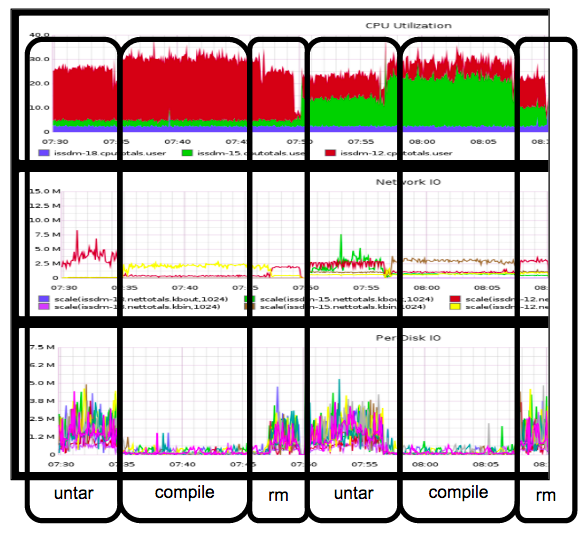
\includegraphics[width=75mm]{figures/creates-motivation.png}
\caption{Create-heavy workloads (untar) incurr the highest disk, network, and CPU
utilization because the metadata server is managing consistency and fault
tolerance.}\label{fig:creates-motivation}
\end{figure}

In our examiniation of the overheads of POSIX we benchmark and analyze CephFS,
the file system that uses the RADOS object store to store its data and
metadata. We choose CephFS because it is an open-source production quality
system. CephFS made one set of design decisions and we not asserting that the
design decisions that were made are superior but instead highlight the
effect those decisions have on performance.

To show how CephFS behaves under high metadata load we use a create-heavy
workload because these types of workloads incurr high CPU, network, and disk
usage.  Figure~\ref{fig:creates-motivation} shows a compilation of the Linux
kernel, which has a download, untar, compile, and remove phase. The untar phase
is characterized by many creates and has the highest resource usage, indicating
that it is stressing the consistency and journalling subsystems of the metadata
server. Also of note: a create-heavy workload does not help for caching indoes.

In this section, we quantify the costs of consistency and fault tolerance in
CephFS. If the components that ensure these semantics (i.e. capabilities and
journals, respectively) can be mitigated or delayed, then global namespaces
perform as well as decoupled namespaces. We run our experiments on a 9 OSD, 3
MDS, 1 MON Ceph cluster. The clients use the Ceph kernel client, which has been
in the mainline Linux kernel since TODO. We use the kernel client so that we
can find the true create speed of the server; our experiments show a low CPU
utilziation for the clients which indicates that we are stressing the servers
more. We also turn caching off becuase, as shown in figureX there is little
difference, in terms of performance between caching and not caching when using
the kernel client.

\subsection{Fault Tolerance}
\label{sec:fault-tolerance}

\begin{figure*}[t]
  \centering
  \begin{subfigure}[b]{.3\linewidth}
      \centering
      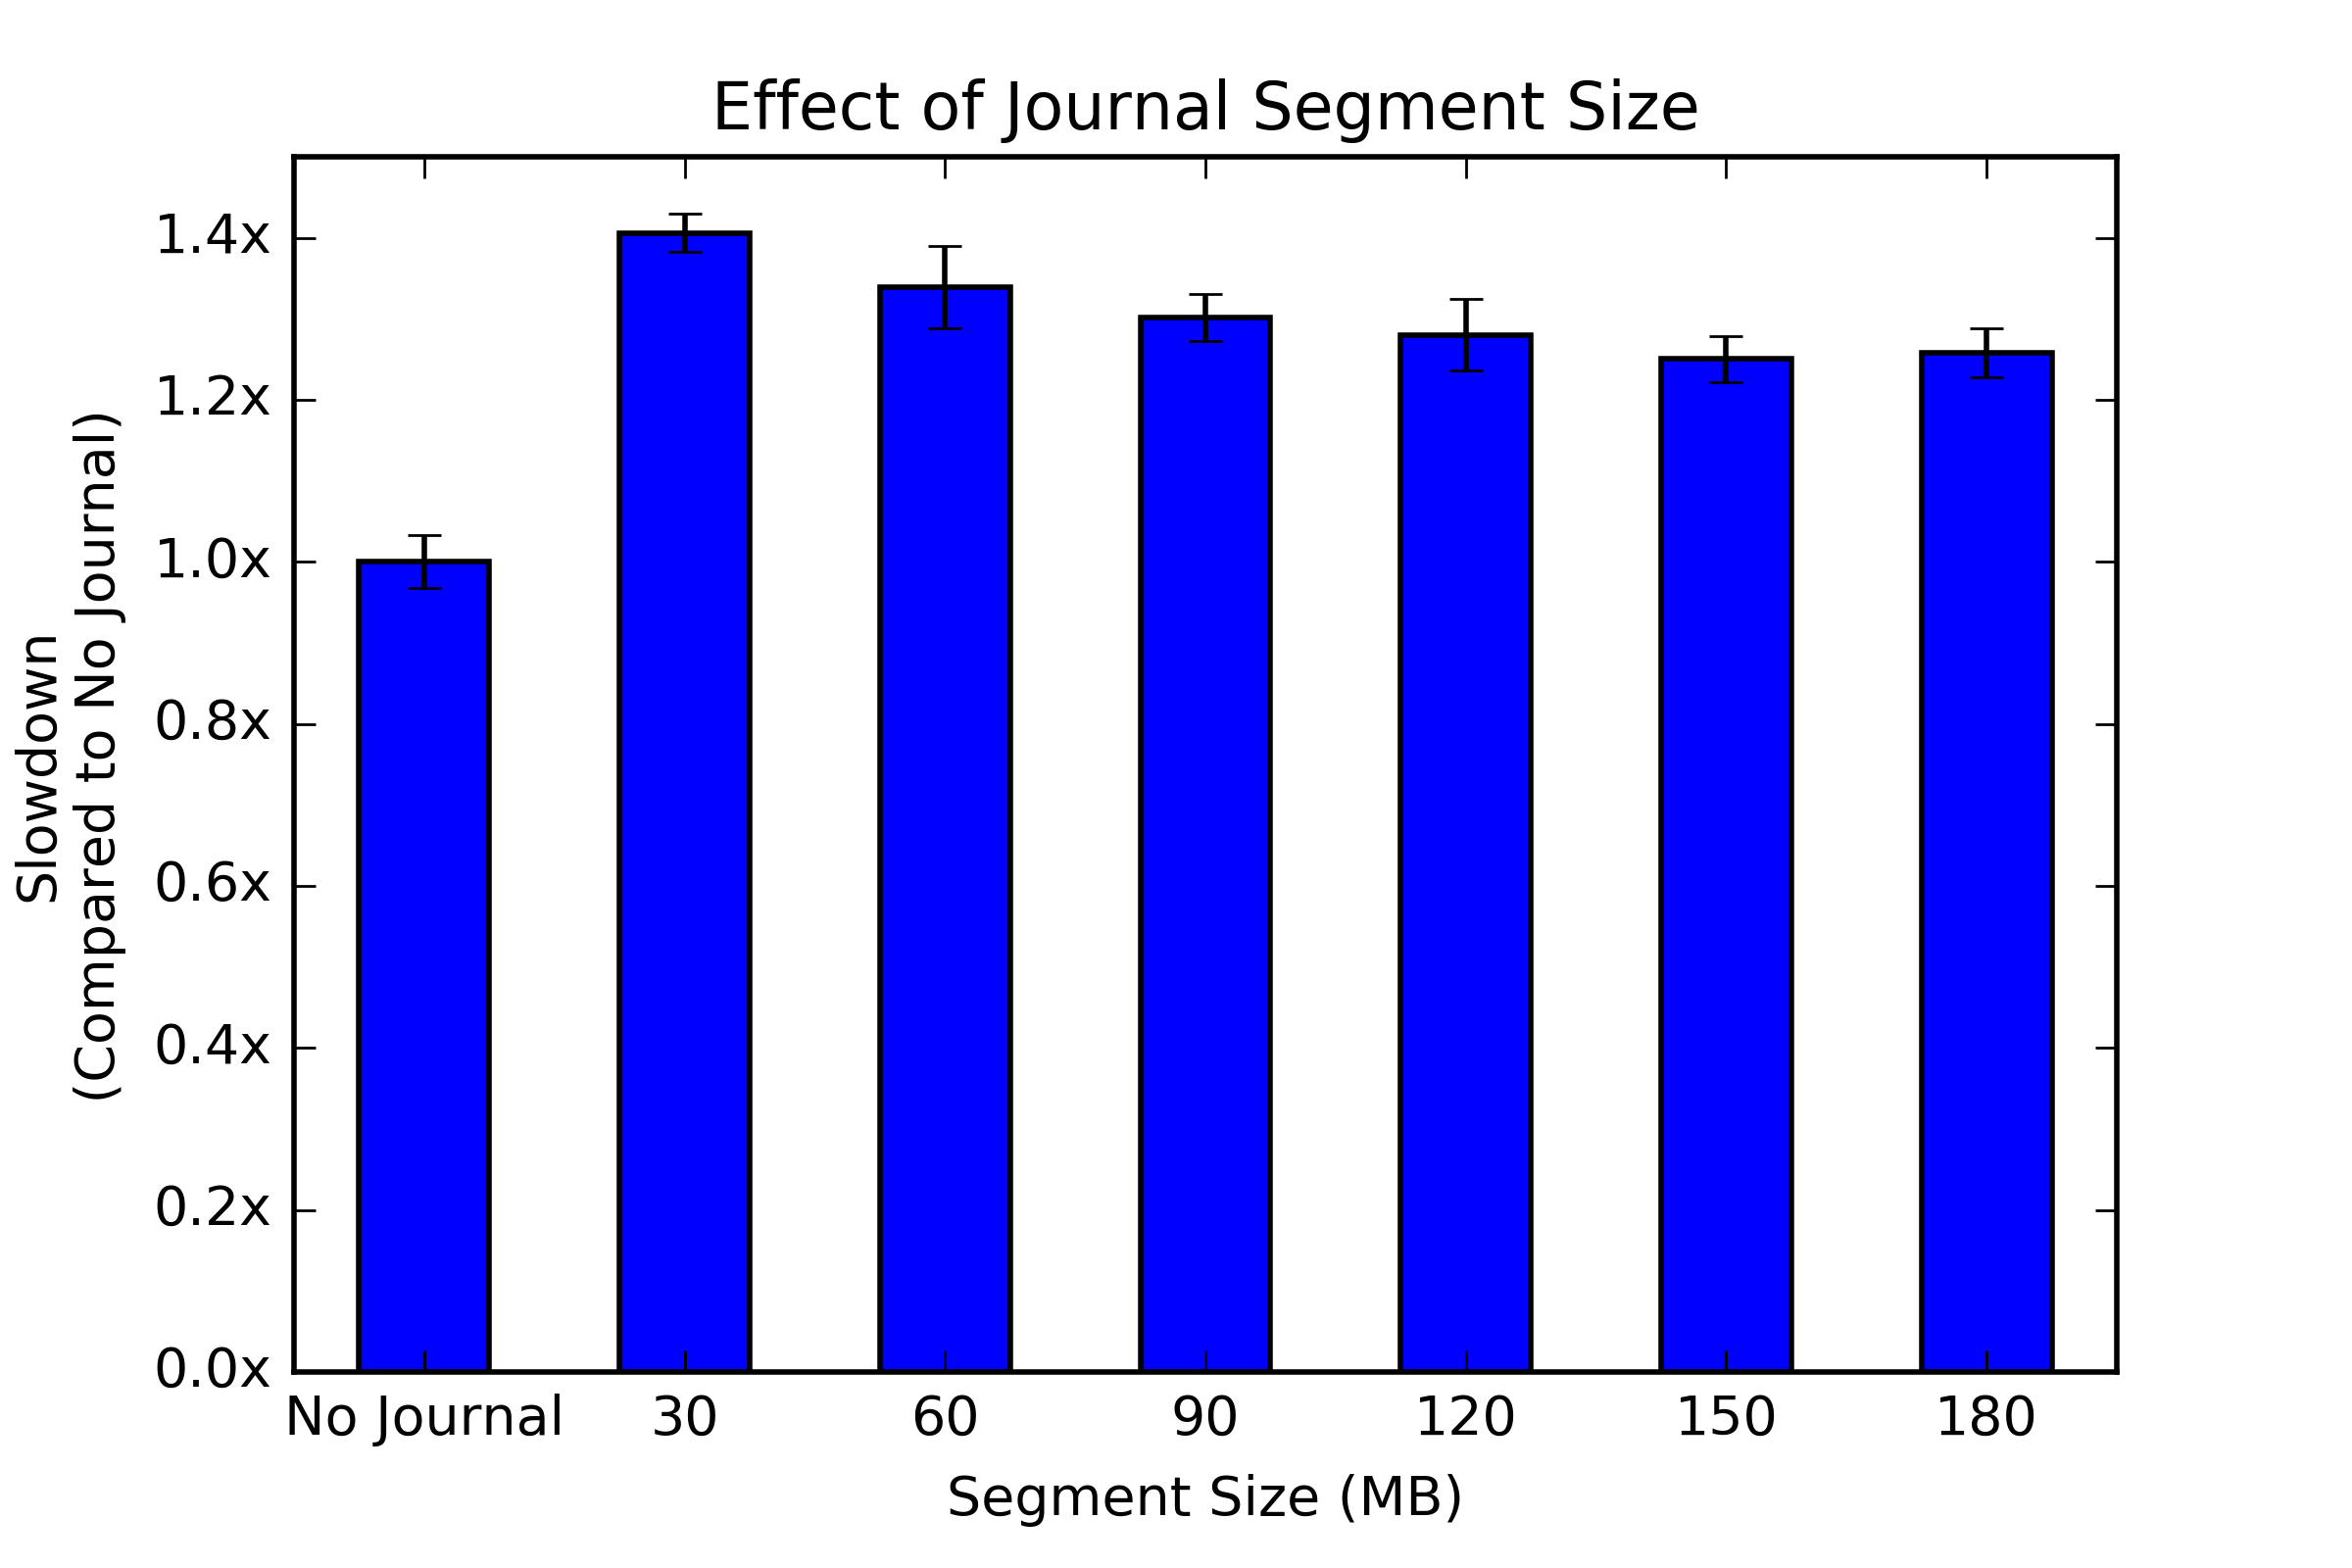
\includegraphics[width=1.0\linewidth]{graphs/slowdown-journal.png}
      \caption{}
      \label{fig:phy-design}
  \end{subfigure}
  \begin{subfigure}[b]{.3\linewidth}
      \centering
      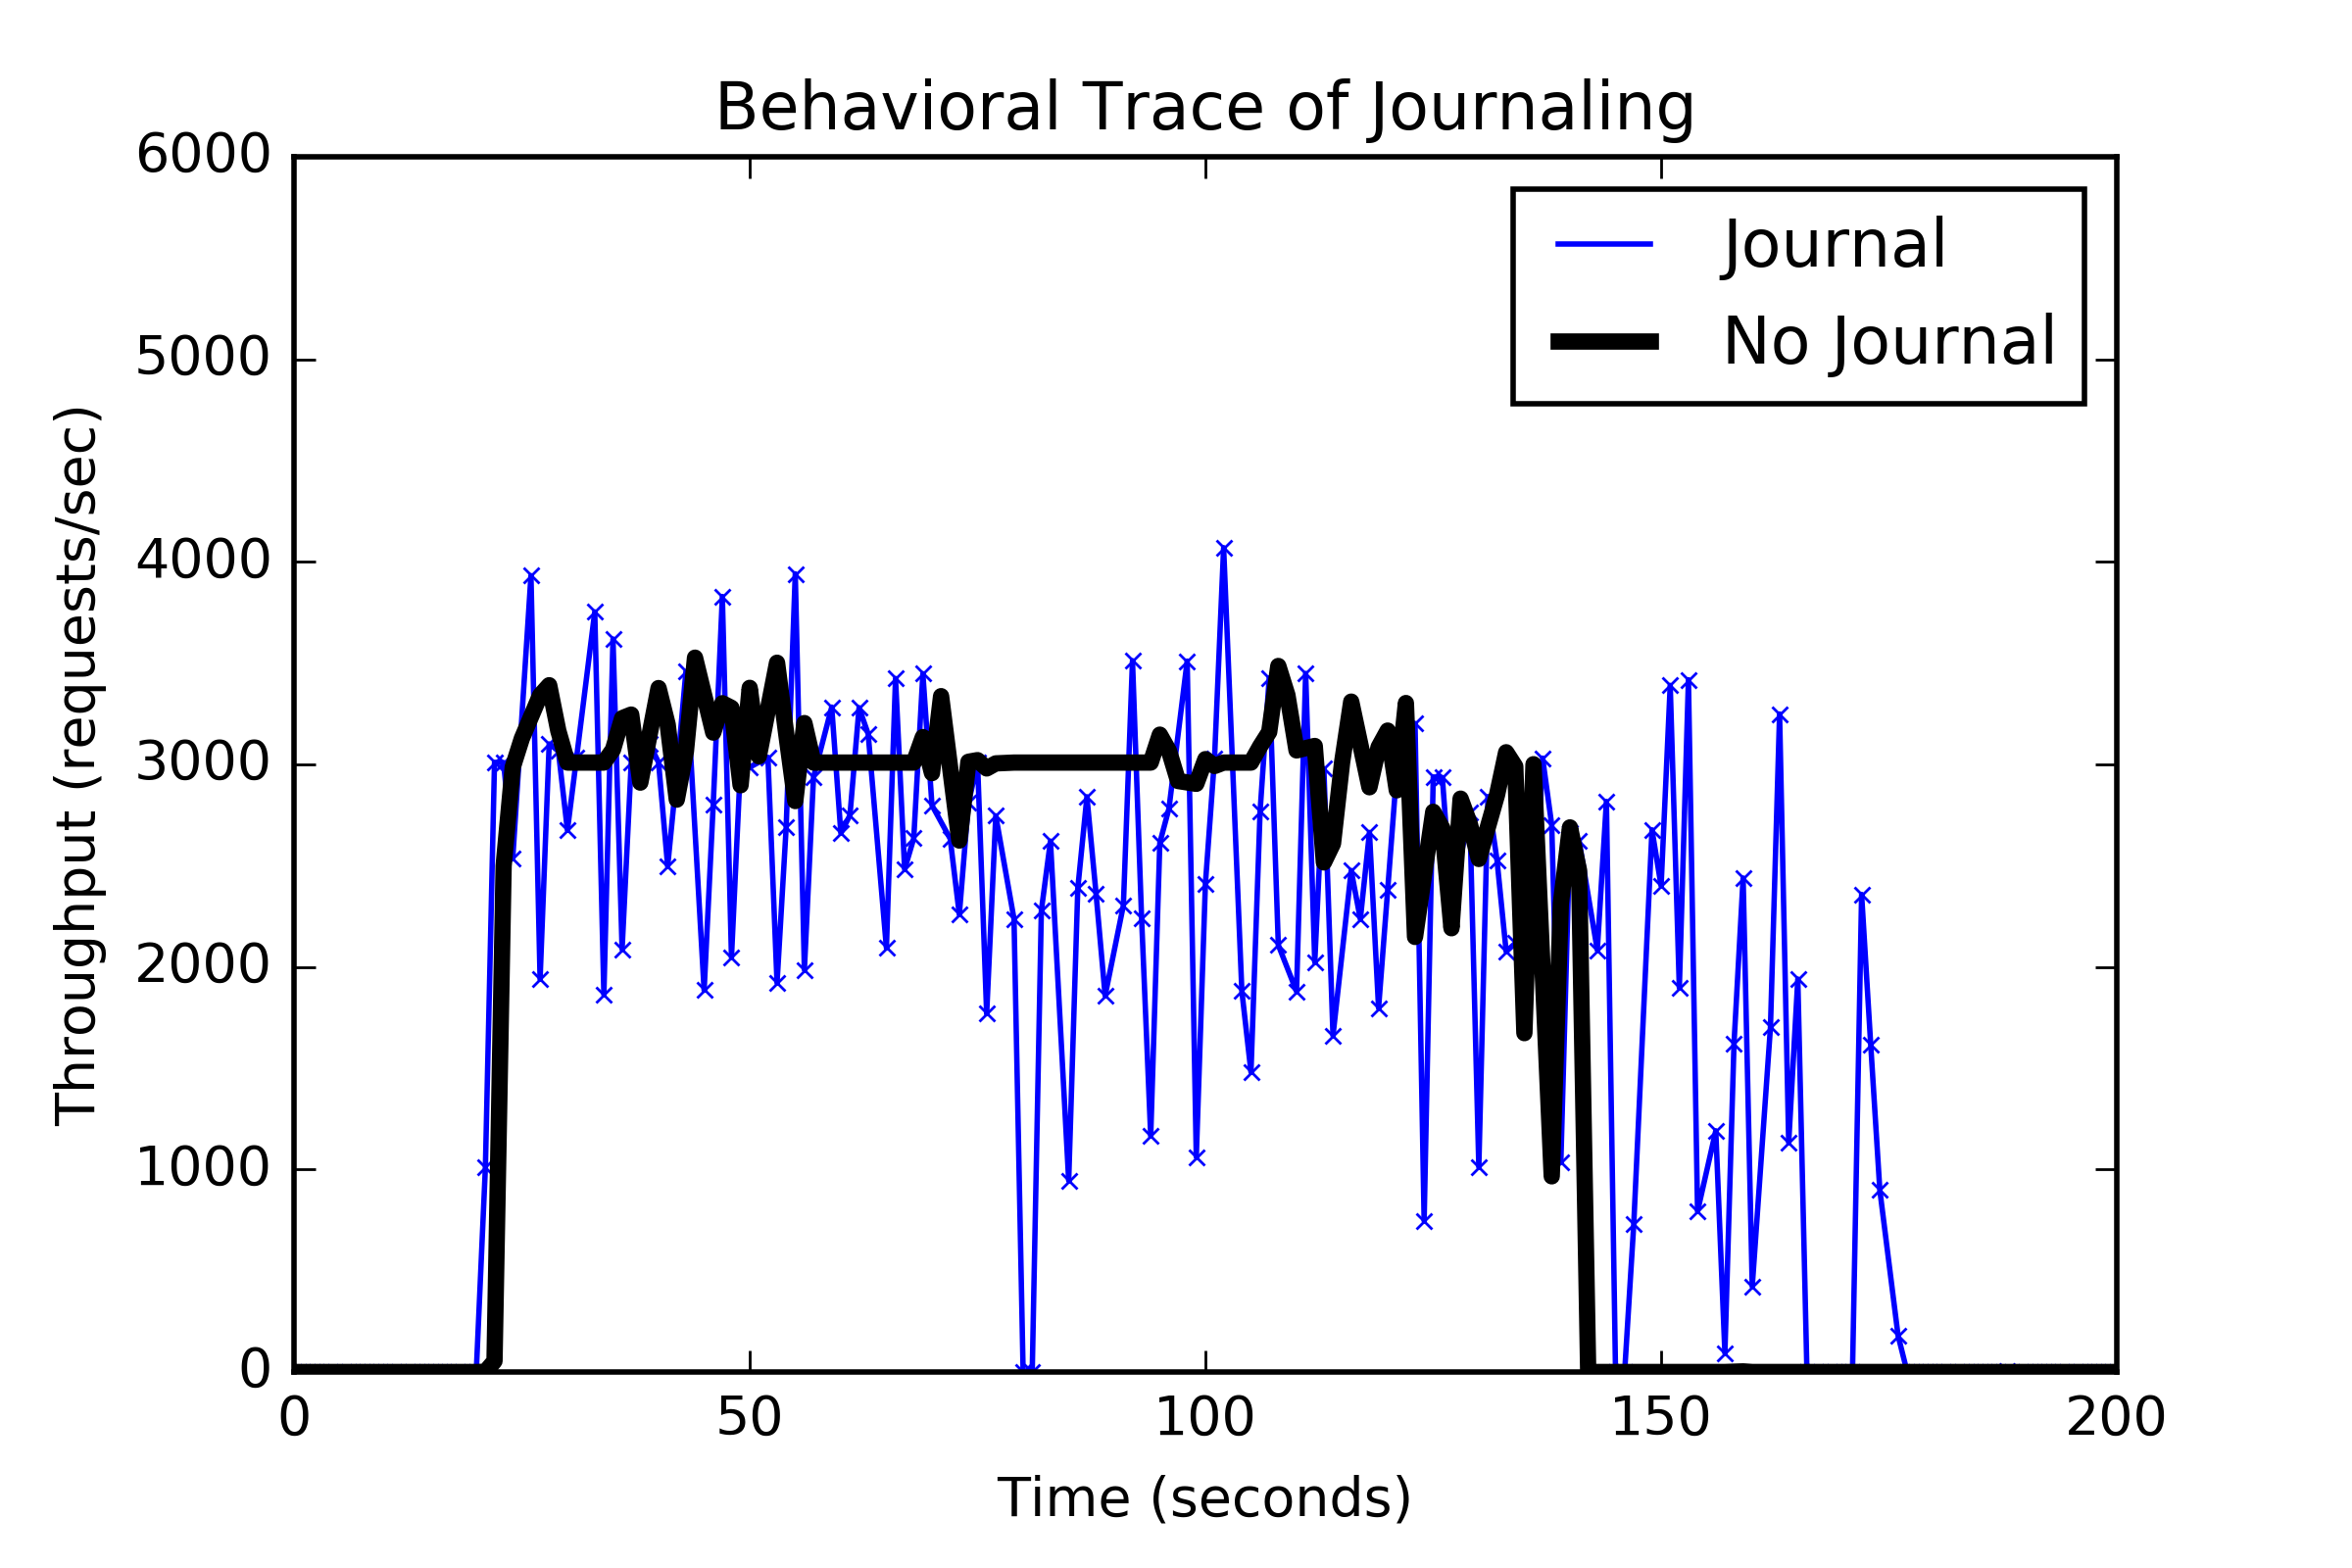
\includegraphics[width=1.0\linewidth]{graphs/behavior-journal.png}
      \caption{}
      \label{fig:batching}
  \end{subfigure}
  \begin{subfigure}[b]{.3\linewidth}
      \centering
      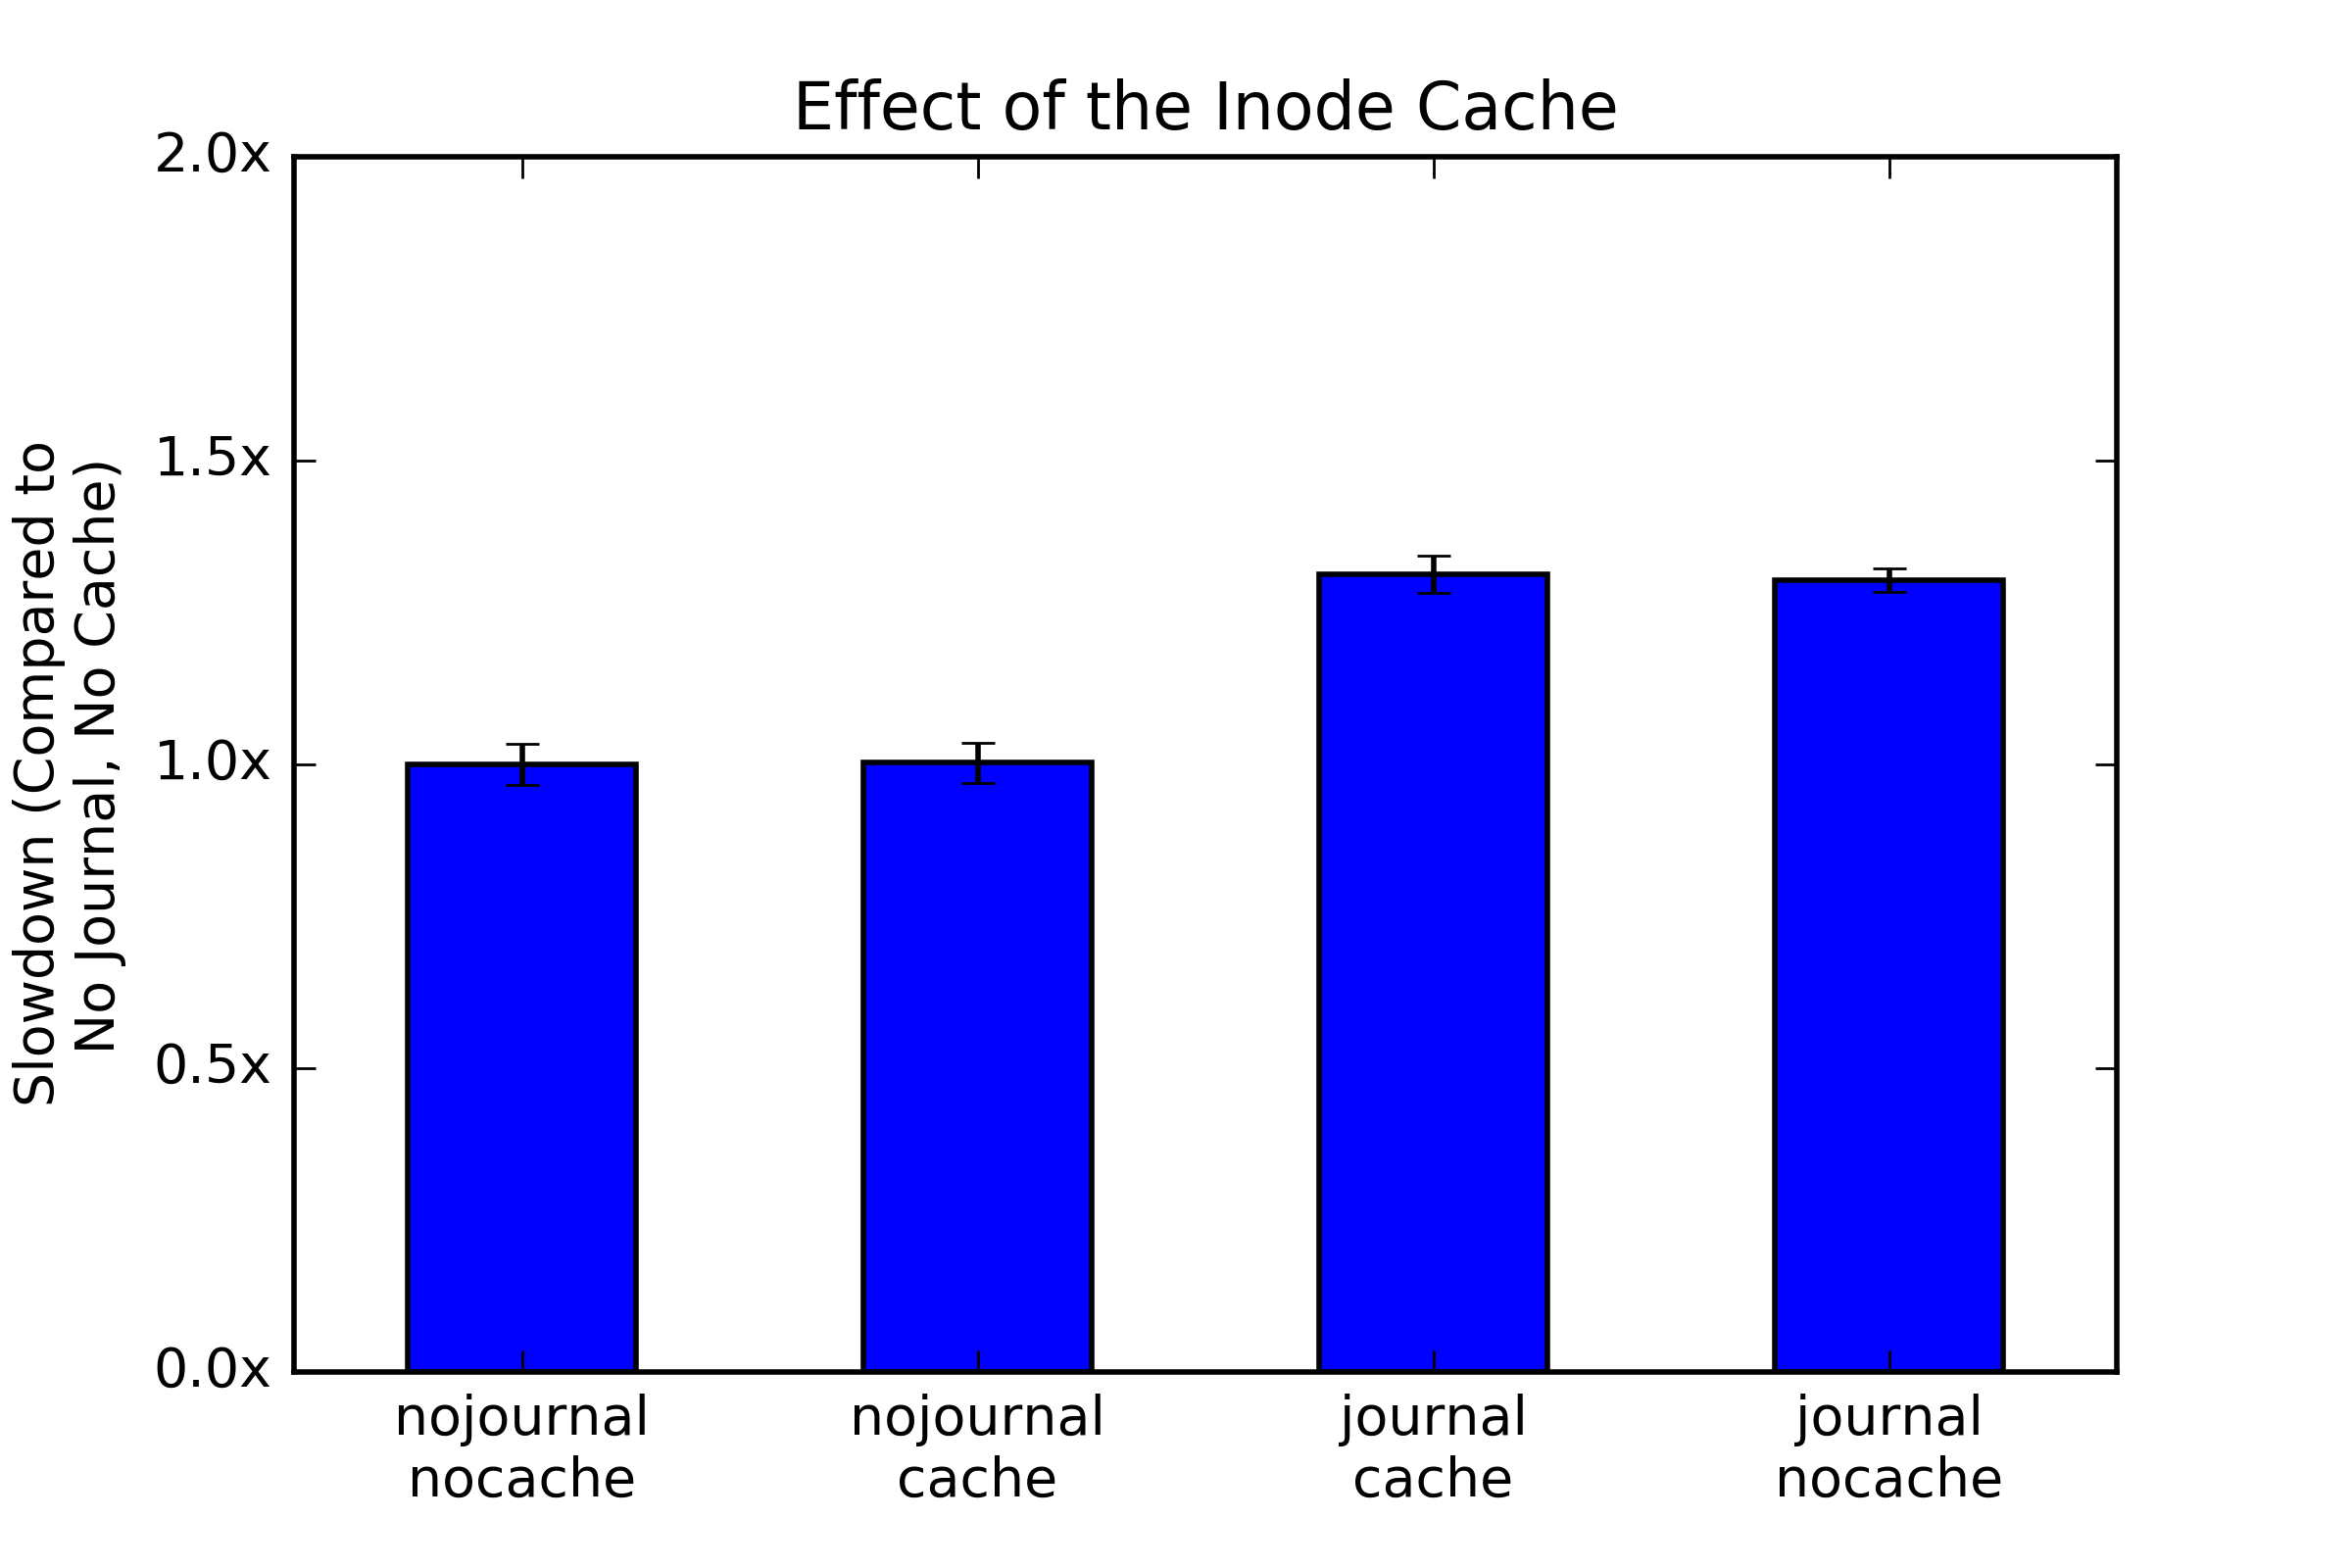
\includegraphics[width=1.0\linewidth]{graphs/slowdown-cache.png}
      \caption{}
      \label{fig:batching-outlier}
  \end{subfigure}
  \caption{(a) relative performance differences are different after storage
  software upgrade. (b) total throughput with and without batching. (c)
  identifying and handling an outlier maintains the benefits
  of batching without the performance degradation of unnecessarily large I/O
  requests.}
\end{figure*}

\begin{figure}[tb] \centering
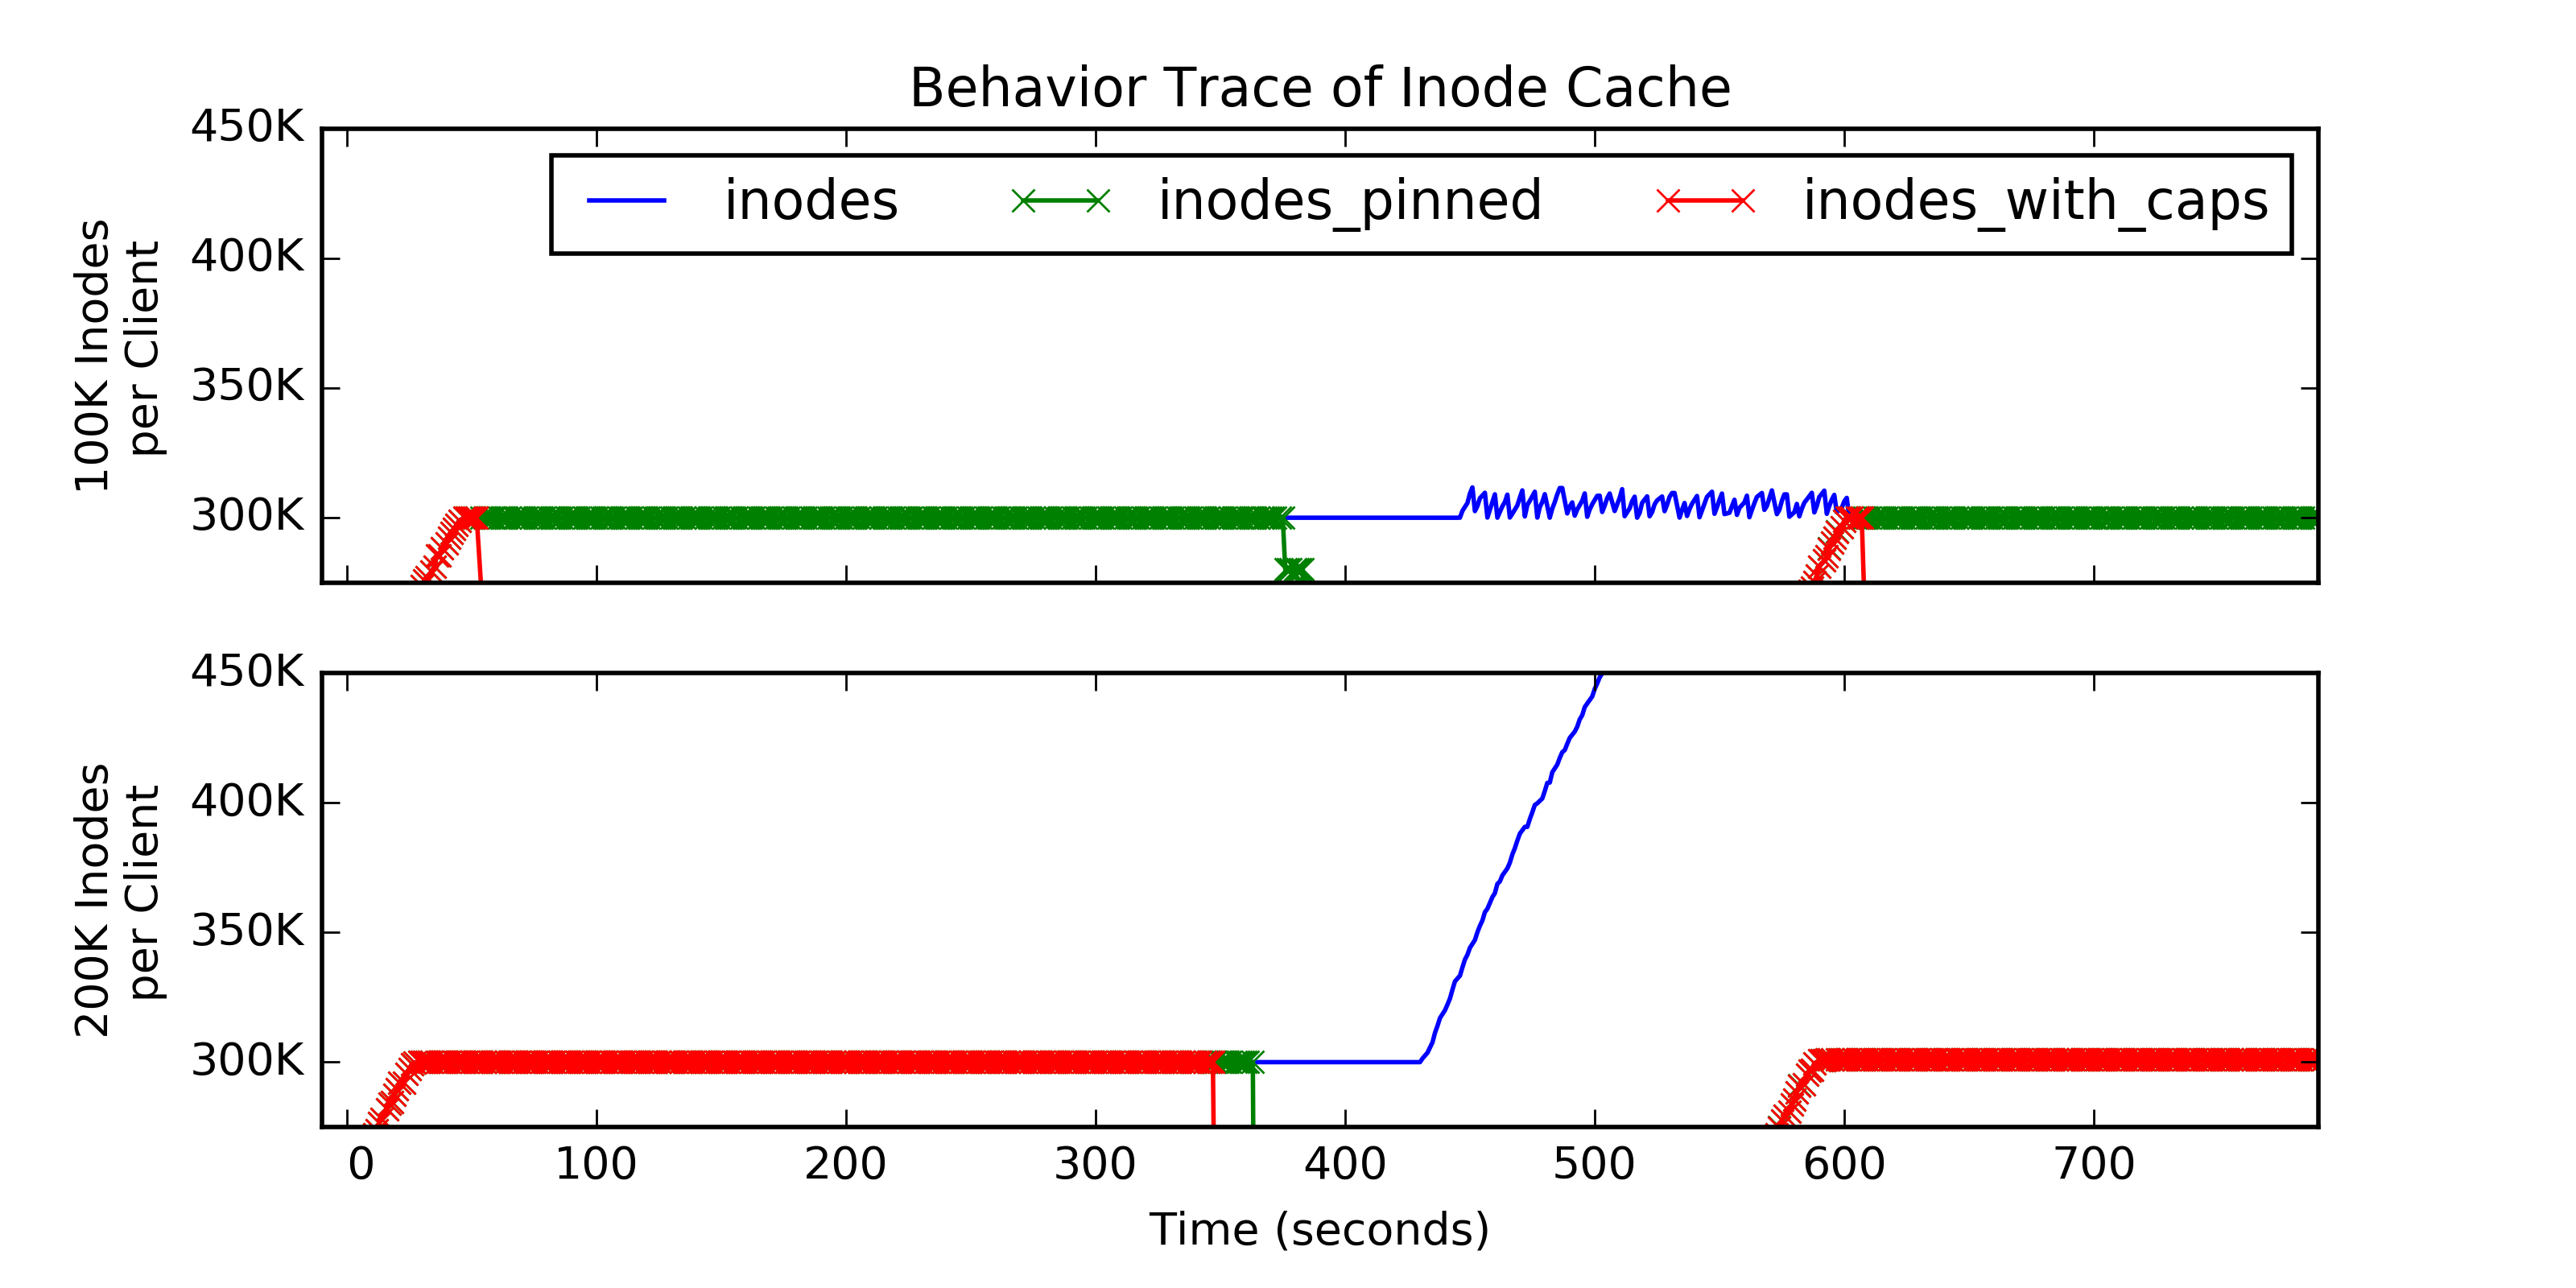
\includegraphics[width=1\linewidth]{./graphs/behavior-cache.png} 
\caption{The inode cache improves metadata read performance but for our
create-heavy workload it is only an overhead. Most of the time maintaining the
cache is spent evicting and adding inodes.}\label{fig:inode-cache}
\end{figure}

\begin{figure}[tb] \centering
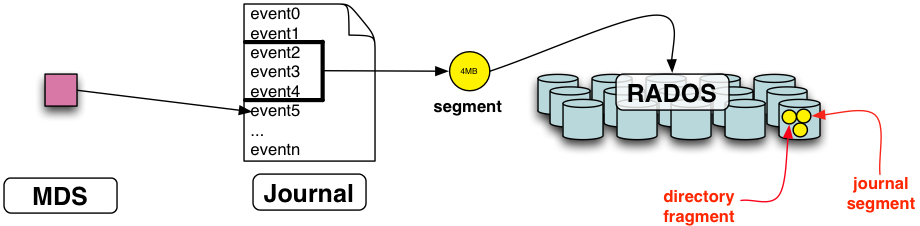
\includegraphics[width=1\linewidth]{./figures/journal.png} 
\caption{CephFS uses a journal to stage updates and tracks dirty metadata in
the collective memory of the MDSs. Each MDS maintains its own journal, which is
broken up into 4MB segments. These segments are pushed into RADOS and deleted
when that particular segment is trimmed from the end of the log. In addition to
journal segments, RADOS also stores per-directory objects. \label{fig:journal}}
\end{figure}

%\begin{figure*}[tb]%h
%\centering
%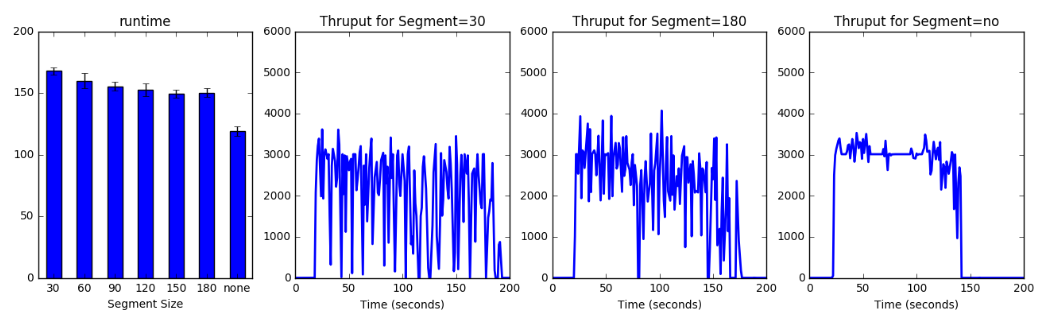
\includegraphics[width=180mm]{figures/throughput-journal.png}
%\caption{Performance improves with larger journal segments because the metadata
%server spends less time flushing the journal }\label{fig:throughput-journal}
%\end{figure*}

%\begin{figure}[tb]%h
%\centering
%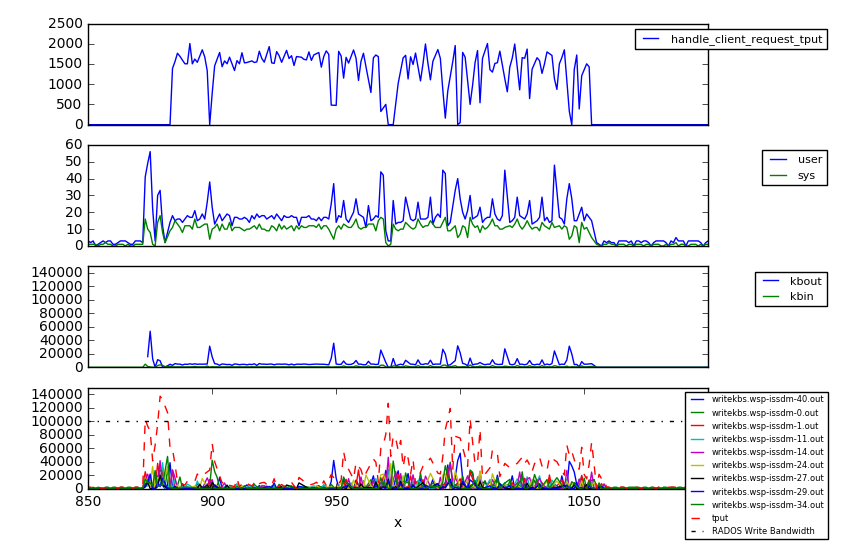
\includegraphics[width=80mm]{figures/throughput-journal-old.png}
%\caption{(a), (b), and (c) show increased activity halfway though the run; (d)
%shows that this activity is related to disk IO, indicating that the activity is
%the journal.  Despite the activity, we conclude that RADOS itself is not the
%bottleneck because our RADOS cluster can sustain 100MB/s write bandwidth.
%}\label{fig:throughput-journal-old}
%\end{figure}
%Figure~\ref{fig:throughput-cache} shows that journaling metadata updates into
%the object store has an overhead.  (a) shows that throughput degrades halfway
%through the run; (b) shows that cpu utilization spikes at this same point; (c)
%shows that outgoing network utilization spikes; and (d) shows that this
%activity spikes on the disks in RADOS.

% purpose of the journal
As shown in Figure~\ref{fig:journal} CephFS uses RADOS (1) as a metadata store
for all information about files including the hierarchical namespace and (2) as
a staging area for the journal of updates before they are applied to the
metadata store. (1) is essentially a cache that improves performance by serving
metadata from memory and (2) is the mechanisms for achieving fault tolerance. 

% - sequential IO, trim redundant operations
Fault tolerance means that the client or server can fail and metadata will not
be lost.  CephFS addresses fault tolerance with a metadata journal that streams
into the resilient object store. Similar to LFS~\cite{} and WAFL~\cite{} the
metadata journal can grow to large sizes ensuring (1) sequential writes into
RADOS and (2) the ability for daemons to trim redundant or irrelevent journal
entries. 

% Knobs in CephFS
The journal is striped over objects where multiple journal updates can reside
on the same object. There are two tunables for controlling the journal: the
segment size and the number of parallel segments that can be written in
parallel. The former is memory bound as larger segments take up more memory but
can reduce the time spent journaling and the latter is CPU bound. 

% Effects on performance
Figure~\ref{fig:throughput-journal} shows that journaling metadata updates into
the object store has an overhead. Part (a) shows the runtime for different
journal segment sizes; the larger the segment size the bigger that the writes
into the object store are. The trade-off comes is in terms of memory because
larger segment sizes take up more space with their buffers. Parts (b), (c), and
(d) show the throughput over time for different segment sizes. Performance
suffers when time is spent journaling. 

% Conclusion
Despite this overhead, we posit that the journal is sufficient to slow down
metadata throughput but not so much as to overwhelm RADOS because we measured
our peak bandwidth to be 100MB/s, which is the speed of our network link.

\textbf{Comparison to decoupled namespaces}: In BatchFS and DeltaFS, as far as
we can tell, when a client or server fails there is no recovery scheme. For
BatchFS, if a client fails when it is writing to the local log-structured
merged tree (implemented as an SSTable) then those batched metadata operations
on lost. For DeltaFS, if the client fails then on restart the computation does
the work again -- since the snapshots of the namespace are never globally
consistent, there is no ground truth the requires the failed namespace to
answer to anyone. On the server side, BatchFS and DeltaFS use IndexFS. Again,
IndexFS writes metadata to SSTables but it is not clear whether they ever
vacate memory, get written to disk, or are flushed to the object store.

\subsection{Strong Consistency} 

Access to POSIX metadata is strongly consistent, so reads and writes are
globally ordered. The synchronization and serialization machinery needed to
ensure that all clients see the same state has high overhead.  CephFS uses
capabilities to keep metadata strongly consistent. To reduce the number of RPCs
needed for consistency, clients can obtain capabilities for reading, reading
and updating, reads caching, writing, buffering writes, changing the file size,
and performing lazy IO.

\begin{figure*}[t]
  \centering
  \begin{subfigure}[b]{.3\linewidth}
      \centering
      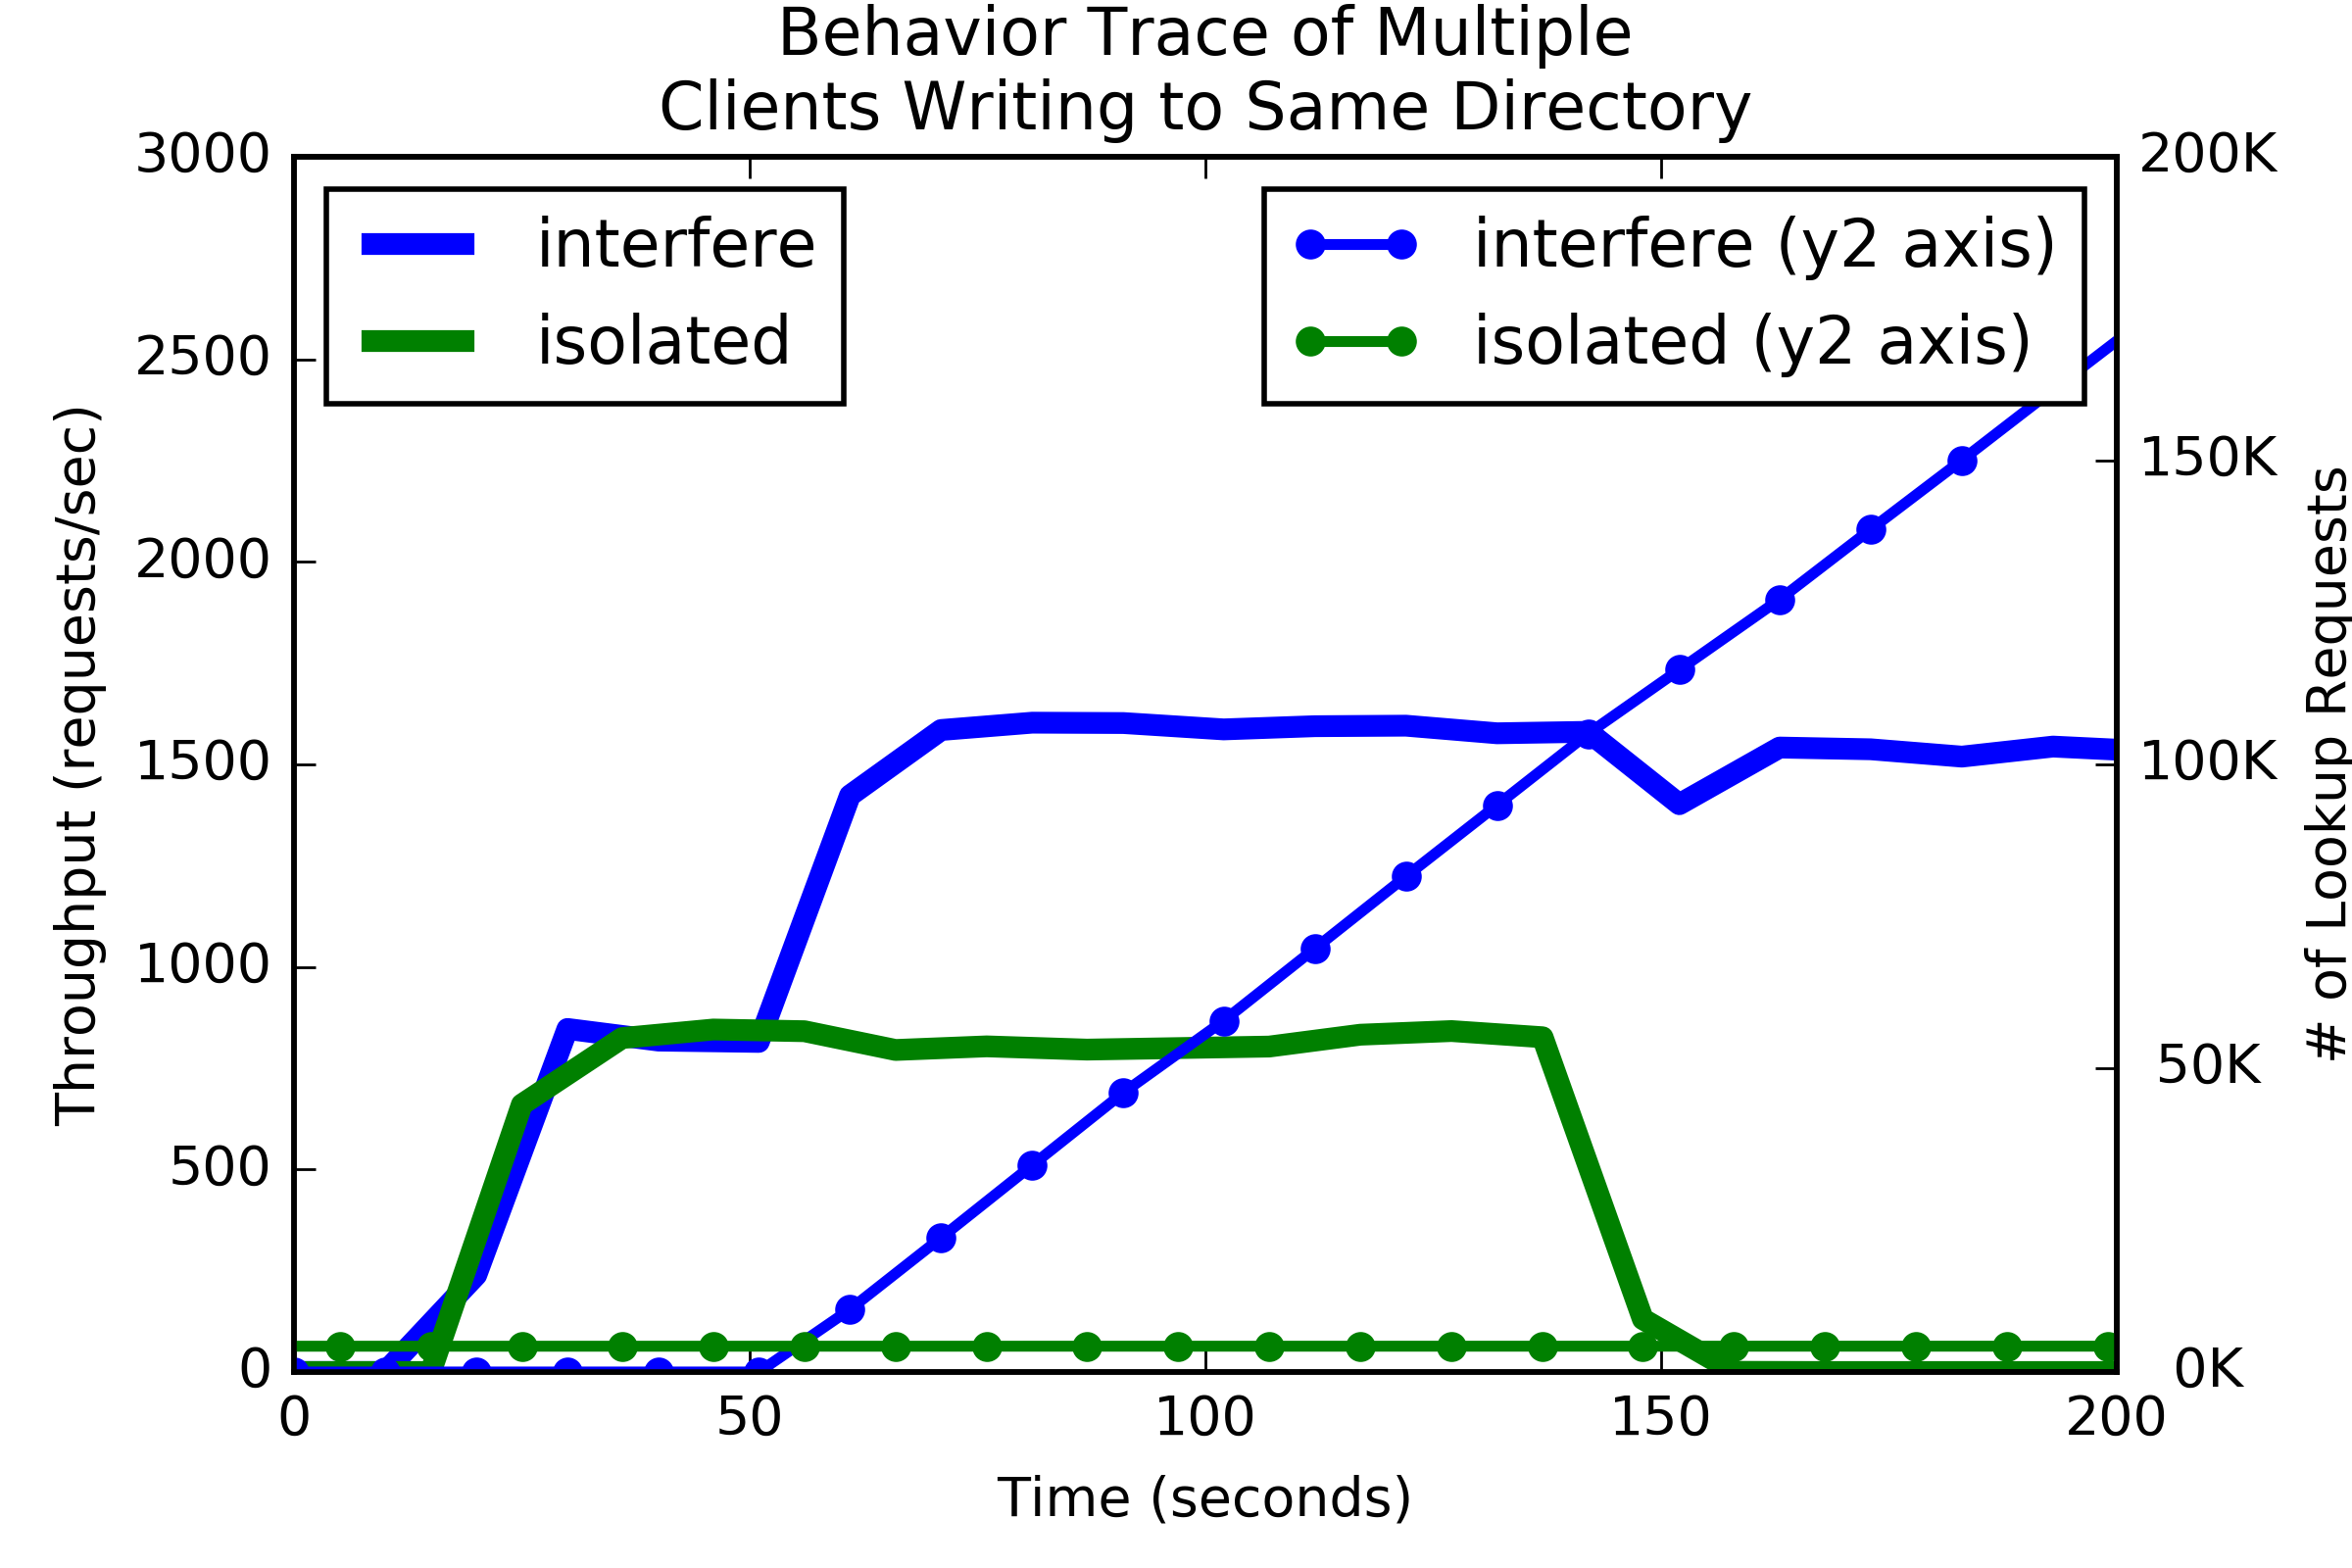
\includegraphics[width=1.0\linewidth]{graphs/behavior-interfere.png}
      \caption{}
      \label{fig:phy-design}
  \end{subfigure}
  \begin{subfigure}[b]{.3\linewidth}
      \centering
      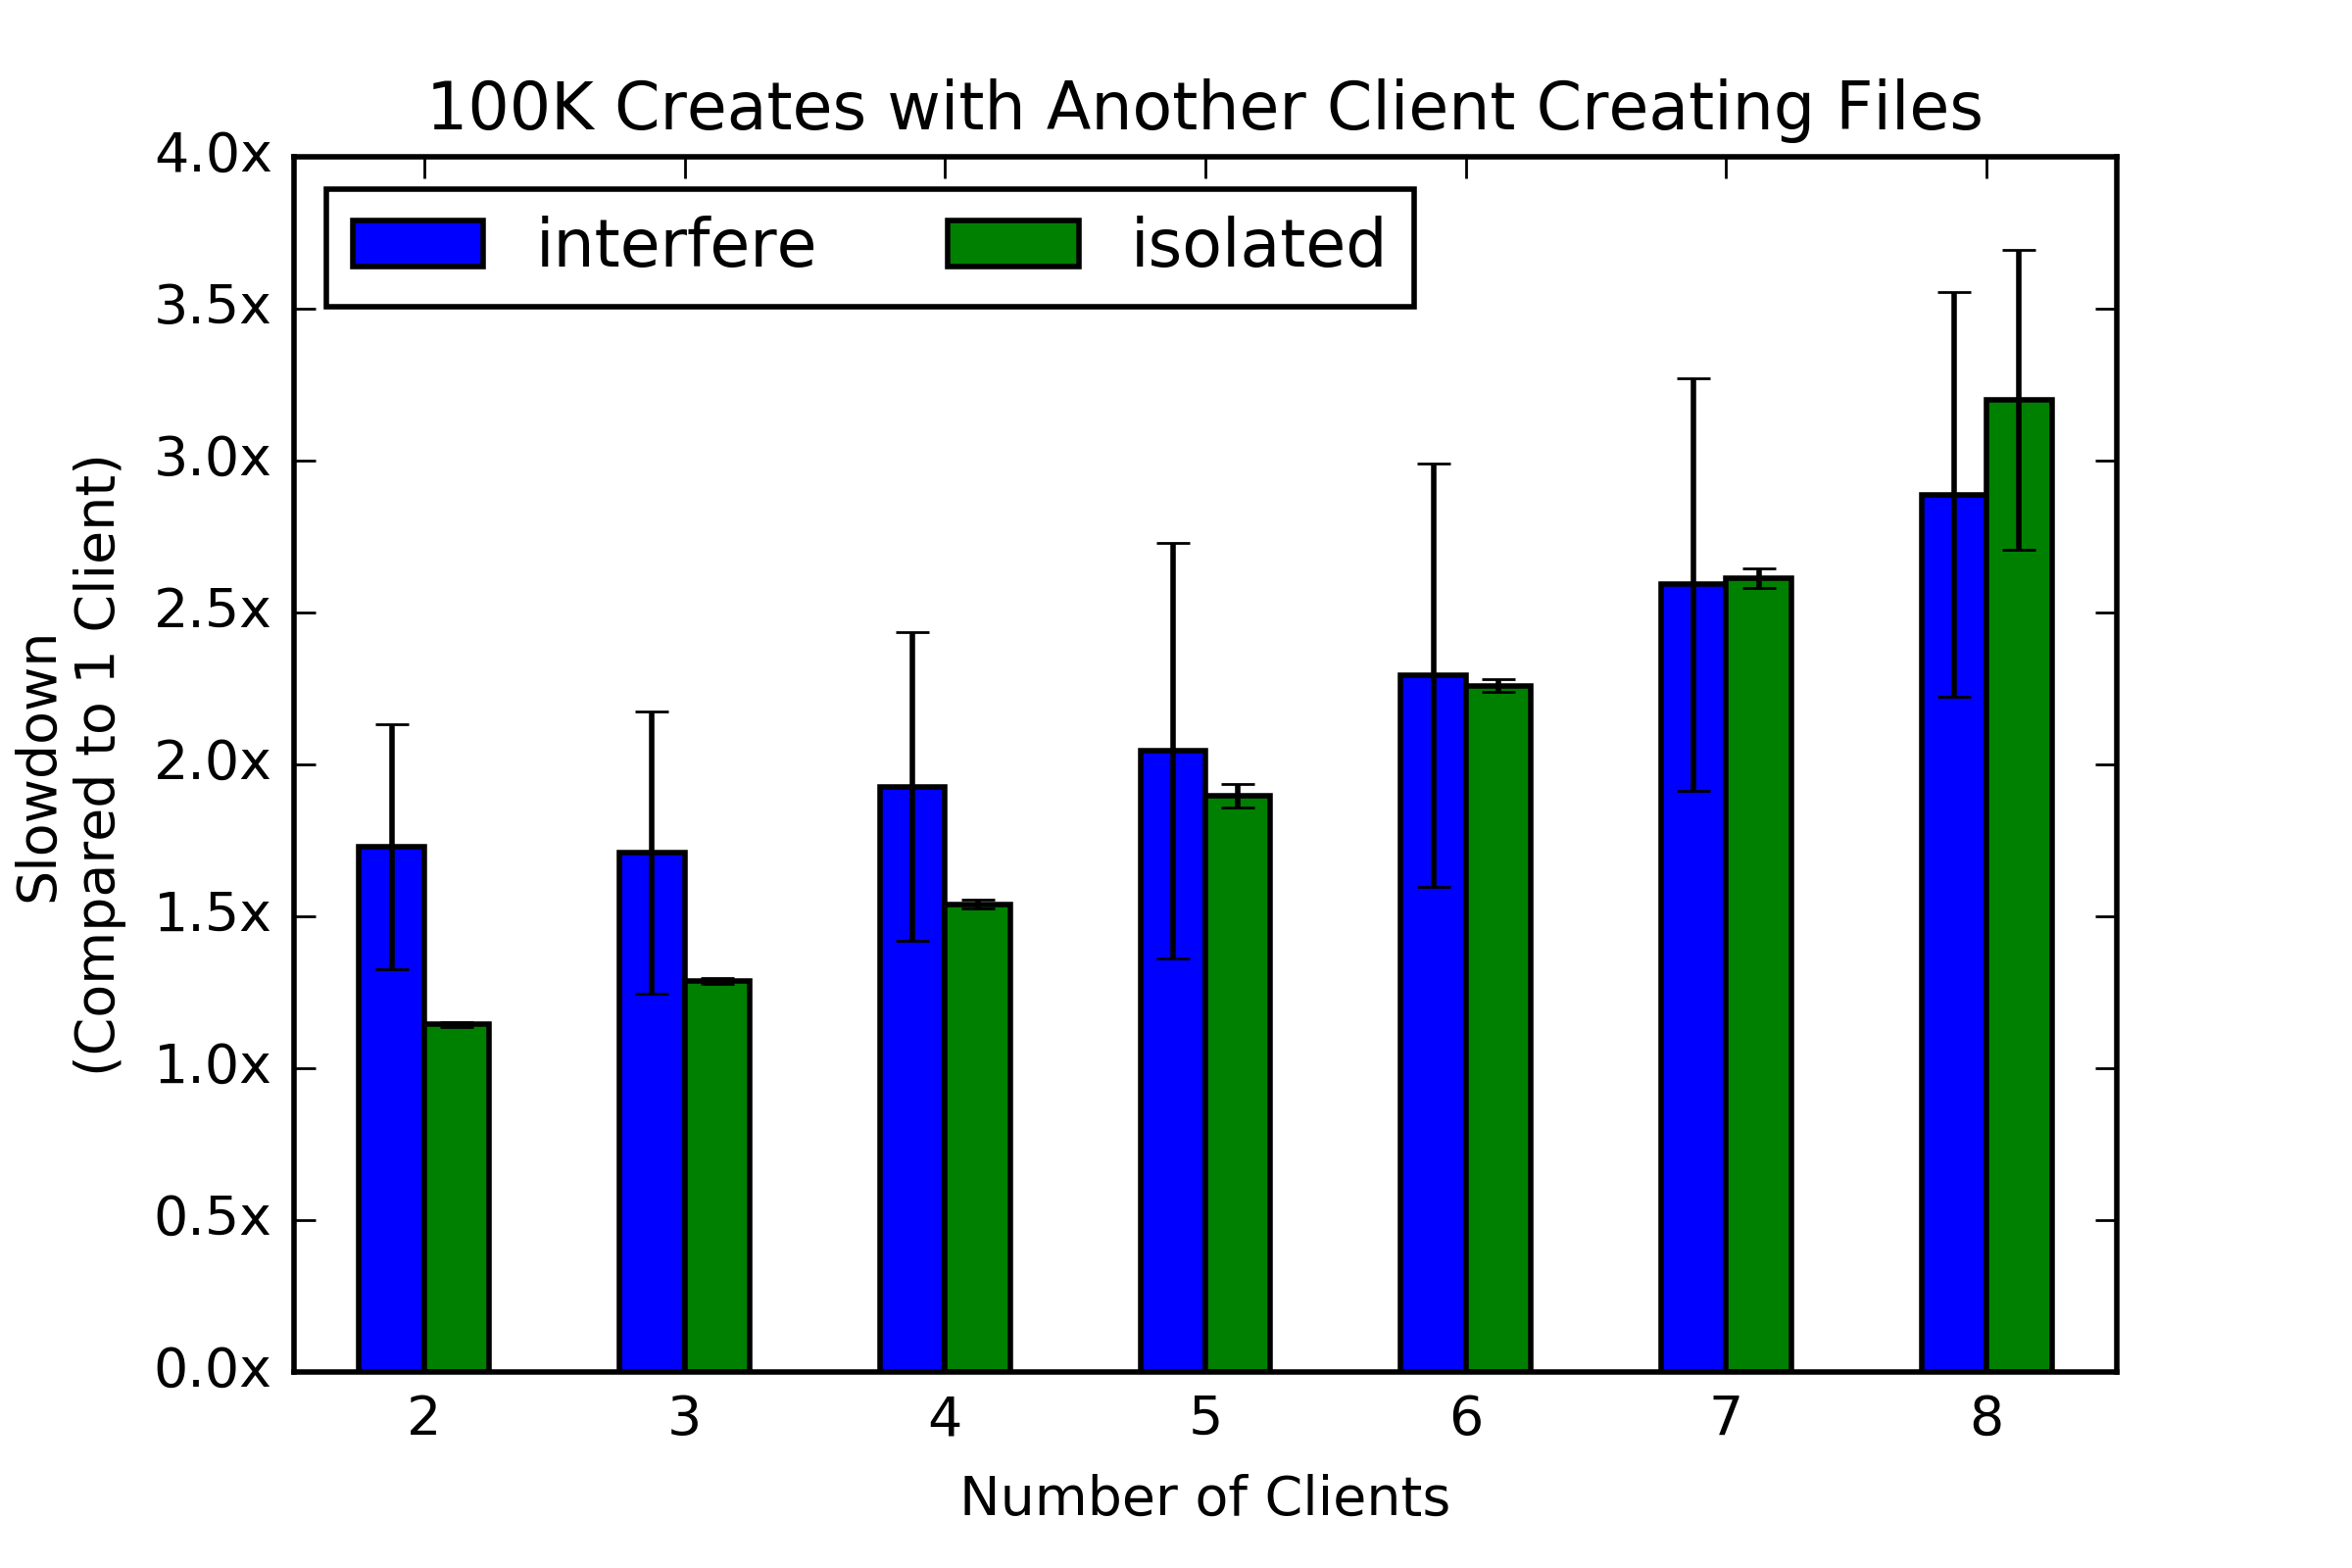
\includegraphics[width=1.0\linewidth]{graphs/slowdown-interfere.png}
      \caption{}
      \label{fig:batching}
  \end{subfigure}
  \begin{subfigure}[b]{.3\linewidth}
      \centering
      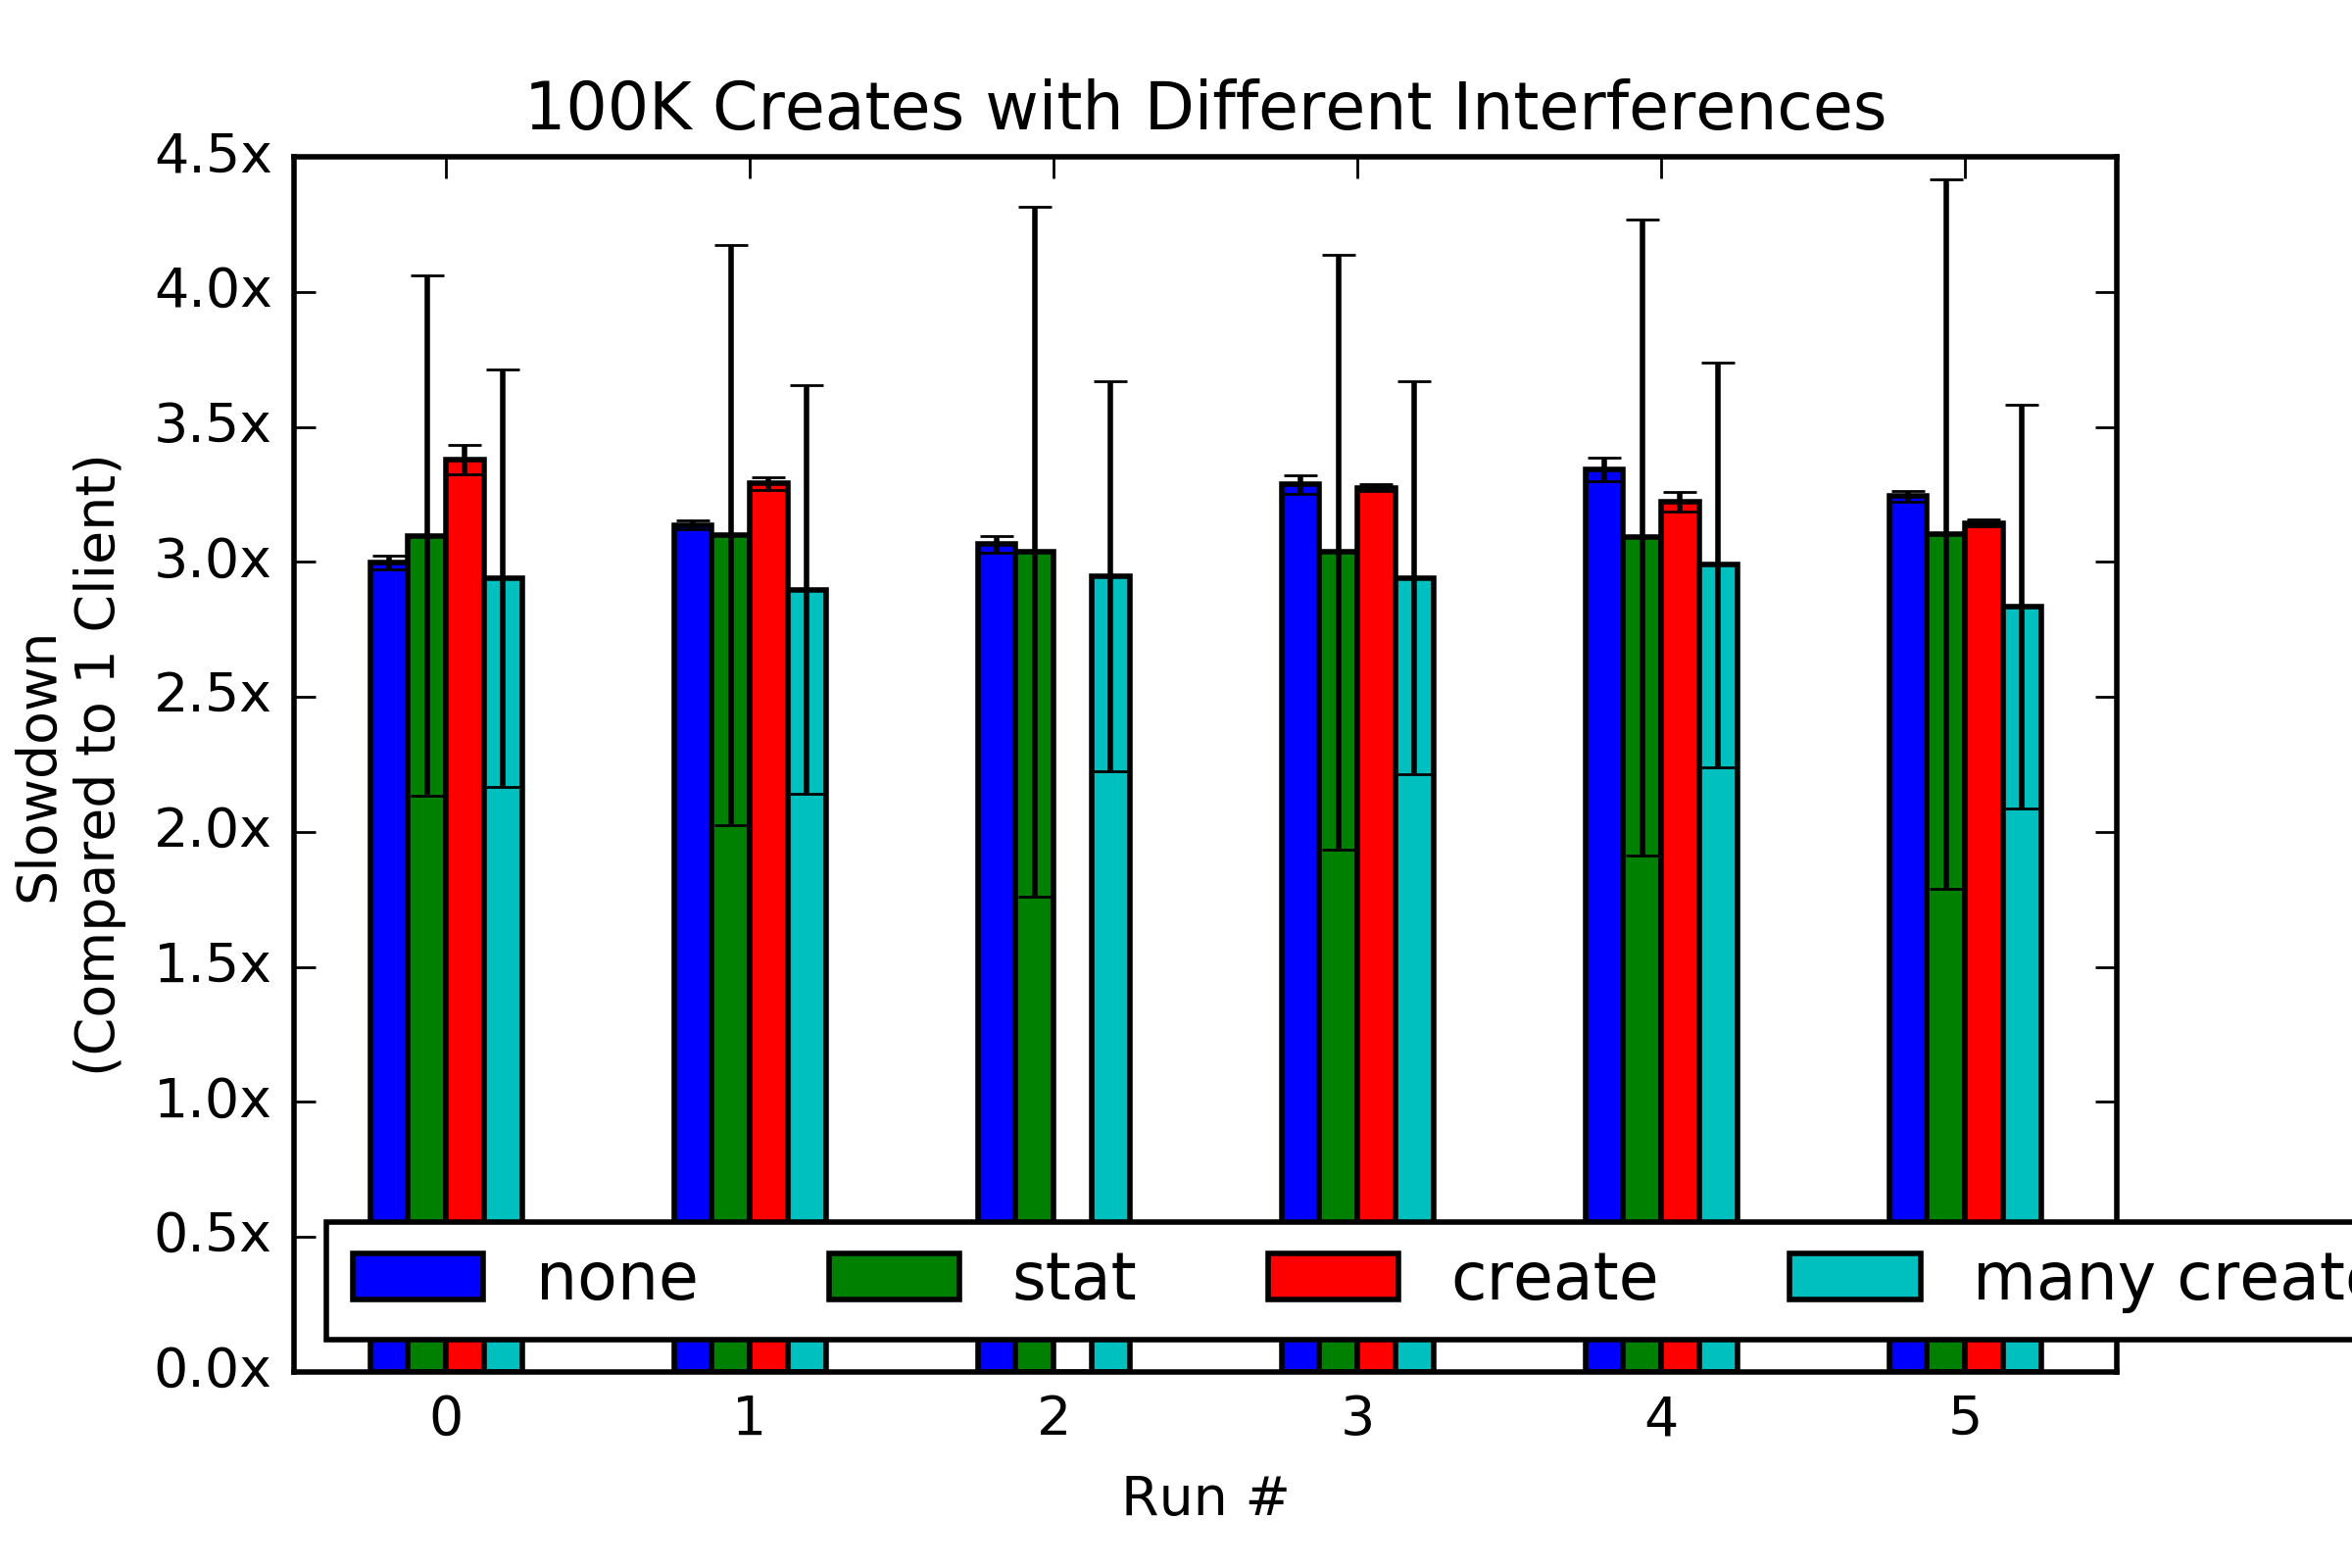
\includegraphics[width=1.0\linewidth]{graphs/slowdown-interfere-types.png}
      \caption{}
      \label{fig:batching-outlier}
  \end{subfigure}
  \caption{When a client create stream is ``isolated" then lookups resolve
  locally but when a second client ``interferes" by creating in the same
  directory, the directory inode capability is revoked forcing all clients to
  centralize lookups at the metadata server.  An underloaded metadata server
  adaquately services conflicting clients; the create speeds are similar while
  the interferring operations are limited by the cost of RPCs.  Scaling clients
  shows increased variability when another client interferes; zooming in on runs
  with 7 clients we see that different types of interferring operations have
  different effects on performance variability and predictability.
  \label{fig:throughput-droplease}}
\end{figure*}

% purpose of the inode ccahe - reduces RPCs (lookups for create, readdirs for
% stats)
To keep track of the read caching and write buffering capabilities, the clients
and metadata servers agree on the state of each inode using an inode cache.  If
a client has the directory inode cached it can do metadata writes (e.g.,
create) with a single RPC. If the client is not caching the directory inode
then it must do multiple RPCs to the metadata server to (1) determine if the
file exists and (2) do the actual create.  Unless the client immediately reads
all the inodes in the cache, the inode cache is less useful for create-heavy
workloads because the cached inodes are unused. 

% benefits
The benefits of caching the directory inode when creating files is shown in
Figure~\ref{fig:throughput-droplease}(a).  If only one client is creating files
in a directory (``isolated" curve) then that client can lookup the existence of
new files locally before issuing a create request to the metadata server. If
another client starts creating files in the same directory (``interfere" curve)
then the directory inode transitions out of read caching and the first client
must send lookups to the metadata server. When other clients interfere the
request throughput is higher Figure~\ref{fig:throughput-droplease}(b) but the
runtime is slower because the isolated client scenario incurrs less requests.
Figures~\ref{fig:throughput-droplease}(c) and (d) plot the creates and lookups,
repsectively, over time; creates slow down and lookups dominate the request
load when the directory inode is shared in the interferring client scenario.

% TODO: what is the cost of trimming the cache?
% TODO: does CephFS still cache inodes when I turn off caching? Why is still keeping inodes in memory? Gah!
%\begin{figure}[tb]%h
%\centering
%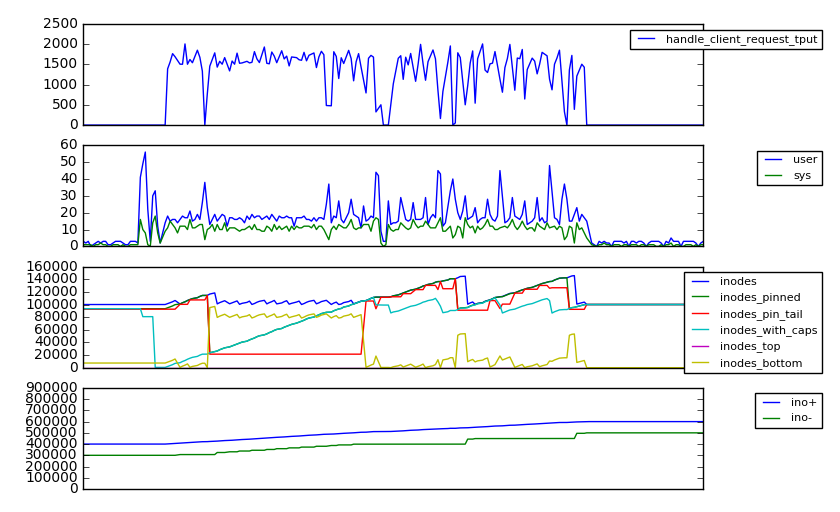
\includegraphics[width=80mm]{figures/throughput-cache.png}
%\caption{ CephFS tries to maintain 100 thousand inodes in the cache;
%performance degrades when it cannot evict inodes fast enough to maintain this
%threshold. \label{fig:throughput-cache}}
%\end{figure}

% disadvantages
The drawbacks of the inode cache are shown in
Figure~\ref{fig:throughput-cache}.  Figure~\ref{fig:throughput-cache}(a) shows
the throughput in metadata requests per second for a single client creating 200
thousand files. Until time 950 the throughput is steady at just under 2000
ops/sec and the CPU utilization is at about 30\%. At time 950 seconds
throughput degrades which corresponds to more inodes in the cache
(Figure~\ref{fig:throughput-cache}(c)). The values in
Figure~\ref{fig:throughput-cache}(c) are:

\begin{itemize}
  \item inodes: total number of elemnts in the cache
  \item inodes pinned: 
  \item inodes pinned tail
  \item inodes with caps
  \item inodes top
  \item inodes bottom 
\end{itemize}

% how the inode cache works
CephFS tries to keep the cache at 100 thousand inodes so the degradation in
performance indicates that the metadata server cannot keep up with the
workload. Figure~\ref{fig:throughput-cache}(d) shows inodes getting added at
the same rate as before 950 seconds (ino\(+\)) but the rate at which inodes get
removed is less stable (ino\(-\)) indicating that cache eviction is taking more
of the metadata servers time.

\subsection{Consistency Overhead}

Figure~\ref{fig:exp0-underloaded} is a baseline showing that the metadata
server can service multiple clients when it is underloaded. One client creates
files in the same directory and another does a touch or stat 15 seconds into
the run. Figure~\ref{fig:exp0-underloaded}(a) shows the runtime of the client
doing the creates: "isolated" is when the create client is the only workload in
the cluster, "interfere stat" is the runtime of the create client when another
client does a stat, and "interfere touch" is the runtime of the create client
when another client does a touch. There is only a minor performance
degradation. Figure~\ref{fig:exp0-underloaded}(b) compares the baseline
the other client doing the touch or stat
%
%and Figure~\ref{fig:exp0-underloaded}
%has a throughput trace to show behavior.
%
%In Figure~\ref{fig:exp0-underloaded}(a), 
%creates only see a minor performance
%degradation while the interferring operations in
%Figure~\ref{fig:exp0-underloaded}(b) show a larger (yet not significant)
%discrepency. 
%
%
%
% isolated is when there is no interferrence from client 1.
To explain Figure~\ref{fig:exp0-underloaded}(a) we use
Figure~\ref{fig:exp0-behaviour}(b) to show why the runtime of creating 100
thousand files is unaffected. Compared to the throughput without an
interferring stat ("isolated" curve) the throughput of the metadata server with
an interferring stat ("inteferring stat" curve) is higher. This means the
metadata server is doing more operations suggesting that it can adequately
handle the demands of both workloads.  

To explain Figure~\ref{fig:exp0-underloaded}(b) we use
Figure~\ref{fig:exp0-underloaded}(a) to show that operations are bounded by the
number of files; more files incurr more requests since both operations lookup
every file. The number of files shown in Figure~\ref{fig:exp0-behaviour}(a)
indicates that the local stat ("client 0" bar) is interacting with less files
than the remote stat ("client 1" bar). This graph also explains why the
isolated stats and touches take the longest from the remote clients; out of all
setups, the isolated operations are doing the most RPCs.  The difference
between local ("client 0 interfere" bar) and remote ("client 1 interfere" bar)
in Figure~\ref{fig:exp0-underloaded}(b) is the overhead of doing RPCs.
Isolated is the slowest because it requests the most files. On average the
local interferring client ("client 0" bar in
Figure~\ref{fig:exp0-behaviour}(a)) requests 40 thousand less files than the
remote interferring call ("client 1" bar in
Figure~\ref{fig:exp0-behaviour}(a)). This reflects how fast the local client
can get into the queue of requests, presumably because it bypasses capability
checks.

From this experiment we make 2 conclusions: (1) the metadata server is not
overloaded because it can handle both workloads and (2) the metadata server
needs to get global consistency from only 1 client

\textbf{Comparison to decoupled namespaces}: Decoupled namespaces merge batches
of metadata operations into the global namespaces when the job completes.  In
BatchFS the merge is delayed by the application using an API to switch between
asynchronous to sychronous mode. The merge itself is explicitly managed by the
application but future work looks at more automated methdologies. In DeltaFS
snapshots of the metadata subtrees stays on the client machines; there is no
ground truth and consistent namespaces are constructed and resolved at
application read time or when a 3rd party system (e.g., middleware, scheduler,
etc.) needs a view of the metadata.


